% Options for packages loaded elsewhere
\PassOptionsToPackage{unicode}{hyperref}
\PassOptionsToPackage{hyphens}{url}
\documentclass[
]{book}
\usepackage{xcolor}
\usepackage{amsmath,amssymb}
\setcounter{secnumdepth}{5}
\usepackage{iftex}
\ifPDFTeX
  \usepackage[T1]{fontenc}
  \usepackage[utf8]{inputenc}
  \usepackage{textcomp} % provide euro and other symbols
\else % if luatex or xetex
  \usepackage{unicode-math} % this also loads fontspec
  \defaultfontfeatures{Scale=MatchLowercase}
  \defaultfontfeatures[\rmfamily]{Ligatures=TeX,Scale=1}
\fi
\usepackage{lmodern}
\ifPDFTeX\else
  % xetex/luatex font selection
\fi
% Use upquote if available, for straight quotes in verbatim environments
\IfFileExists{upquote.sty}{\usepackage{upquote}}{}
\IfFileExists{microtype.sty}{% use microtype if available
  \usepackage[]{microtype}
  \UseMicrotypeSet[protrusion]{basicmath} % disable protrusion for tt fonts
}{}
\makeatletter
\@ifundefined{KOMAClassName}{% if non-KOMA class
  \IfFileExists{parskip.sty}{%
    \usepackage{parskip}
  }{% else
    \setlength{\parindent}{0pt}
    \setlength{\parskip}{6pt plus 2pt minus 1pt}}
}{% if KOMA class
  \KOMAoptions{parskip=half}}
\makeatother
\usepackage{color}
\usepackage{fancyvrb}
\newcommand{\VerbBar}{|}
\newcommand{\VERB}{\Verb[commandchars=\\\{\}]}
\DefineVerbatimEnvironment{Highlighting}{Verbatim}{commandchars=\\\{\}}
% Add ',fontsize=\small' for more characters per line
\usepackage{framed}
\definecolor{shadecolor}{RGB}{248,248,248}
\newenvironment{Shaded}{\begin{snugshade}}{\end{snugshade}}
\newcommand{\AlertTok}[1]{\textcolor[rgb]{0.94,0.16,0.16}{#1}}
\newcommand{\AnnotationTok}[1]{\textcolor[rgb]{0.56,0.35,0.01}{\textbf{\textit{#1}}}}
\newcommand{\AttributeTok}[1]{\textcolor[rgb]{0.13,0.29,0.53}{#1}}
\newcommand{\BaseNTok}[1]{\textcolor[rgb]{0.00,0.00,0.81}{#1}}
\newcommand{\BuiltInTok}[1]{#1}
\newcommand{\CharTok}[1]{\textcolor[rgb]{0.31,0.60,0.02}{#1}}
\newcommand{\CommentTok}[1]{\textcolor[rgb]{0.56,0.35,0.01}{\textit{#1}}}
\newcommand{\CommentVarTok}[1]{\textcolor[rgb]{0.56,0.35,0.01}{\textbf{\textit{#1}}}}
\newcommand{\ConstantTok}[1]{\textcolor[rgb]{0.56,0.35,0.01}{#1}}
\newcommand{\ControlFlowTok}[1]{\textcolor[rgb]{0.13,0.29,0.53}{\textbf{#1}}}
\newcommand{\DataTypeTok}[1]{\textcolor[rgb]{0.13,0.29,0.53}{#1}}
\newcommand{\DecValTok}[1]{\textcolor[rgb]{0.00,0.00,0.81}{#1}}
\newcommand{\DocumentationTok}[1]{\textcolor[rgb]{0.56,0.35,0.01}{\textbf{\textit{#1}}}}
\newcommand{\ErrorTok}[1]{\textcolor[rgb]{0.64,0.00,0.00}{\textbf{#1}}}
\newcommand{\ExtensionTok}[1]{#1}
\newcommand{\FloatTok}[1]{\textcolor[rgb]{0.00,0.00,0.81}{#1}}
\newcommand{\FunctionTok}[1]{\textcolor[rgb]{0.13,0.29,0.53}{\textbf{#1}}}
\newcommand{\ImportTok}[1]{#1}
\newcommand{\InformationTok}[1]{\textcolor[rgb]{0.56,0.35,0.01}{\textbf{\textit{#1}}}}
\newcommand{\KeywordTok}[1]{\textcolor[rgb]{0.13,0.29,0.53}{\textbf{#1}}}
\newcommand{\NormalTok}[1]{#1}
\newcommand{\OperatorTok}[1]{\textcolor[rgb]{0.81,0.36,0.00}{\textbf{#1}}}
\newcommand{\OtherTok}[1]{\textcolor[rgb]{0.56,0.35,0.01}{#1}}
\newcommand{\PreprocessorTok}[1]{\textcolor[rgb]{0.56,0.35,0.01}{\textit{#1}}}
\newcommand{\RegionMarkerTok}[1]{#1}
\newcommand{\SpecialCharTok}[1]{\textcolor[rgb]{0.81,0.36,0.00}{\textbf{#1}}}
\newcommand{\SpecialStringTok}[1]{\textcolor[rgb]{0.31,0.60,0.02}{#1}}
\newcommand{\StringTok}[1]{\textcolor[rgb]{0.31,0.60,0.02}{#1}}
\newcommand{\VariableTok}[1]{\textcolor[rgb]{0.00,0.00,0.00}{#1}}
\newcommand{\VerbatimStringTok}[1]{\textcolor[rgb]{0.31,0.60,0.02}{#1}}
\newcommand{\WarningTok}[1]{\textcolor[rgb]{0.56,0.35,0.01}{\textbf{\textit{#1}}}}
\usepackage{longtable,booktabs,array}
\usepackage{calc} % for calculating minipage widths
% Correct order of tables after \paragraph or \subparagraph
\usepackage{etoolbox}
\makeatletter
\patchcmd\longtable{\par}{\if@noskipsec\mbox{}\fi\par}{}{}
\makeatother
% Allow footnotes in longtable head/foot
\IfFileExists{footnotehyper.sty}{\usepackage{footnotehyper}}{\usepackage{footnote}}
\makesavenoteenv{longtable}
\usepackage{graphicx}
\makeatletter
\newsavebox\pandoc@box
\newcommand*\pandocbounded[1]{% scales image to fit in text height/width
  \sbox\pandoc@box{#1}%
  \Gscale@div\@tempa{\textheight}{\dimexpr\ht\pandoc@box+\dp\pandoc@box\relax}%
  \Gscale@div\@tempb{\linewidth}{\wd\pandoc@box}%
  \ifdim\@tempb\p@<\@tempa\p@\let\@tempa\@tempb\fi% select the smaller of both
  \ifdim\@tempa\p@<\p@\scalebox{\@tempa}{\usebox\pandoc@box}%
  \else\usebox{\pandoc@box}%
  \fi%
}
% Set default figure placement to htbp
\def\fps@figure{htbp}
\makeatother
\setlength{\emergencystretch}{3em} % prevent overfull lines
\providecommand{\tightlist}{%
  \setlength{\itemsep}{0pt}\setlength{\parskip}{0pt}}
\usepackage[]{natbib}
\bibliographystyle{plainnat}
\usepackage{booktabs}

\usepackage{amsmath}
\usepackage{tikz}
\usetikzlibrary{positioning}
\usepackage{bookmark}
\IfFileExists{xurl.sty}{\usepackage{xurl}}{} % add URL line breaks if available
\urlstyle{same}
\hypersetup{
  pdftitle={Math Explorations},
  pdfauthor={Saviour Elikplim Animdife},
  hidelinks,
  pdfcreator={LaTeX via pandoc}}

\title{Math Explorations}
\author{Saviour Elikplim Animdife}
\date{2025-05-16}

\begin{document}
\maketitle

{
\setcounter{tocdepth}{1}
\tableofcontents
}
\chapter*{Preface}\label{preface}
\addcontentsline{toc}{chapter}{Preface}

\begin{center}\rule{0.5\linewidth}{0.5pt}\end{center}

Here, you will encounter my findings on my journey through the world of mathematics. I hope you find the material rewarding and worth exploring. Cheers!

\href{https://github.com/sneurocode/math-explorations/blob/master/docs/_main.pdf}{Download the PDF version}

© 2025 \emph{Saviour E. Animdife}

\chapter{GCD and LCM 1}\label{gcd-and-lcm-1}

The GCD or greatest common divisor of two natural numbers (positive whole numbers) \(a\) and \(b\) is the largest number that can divide the two numbers without a remainder. For example, if we take \(10\) and \(20\) as our two natural numbers, \(5\) divides both without a remainder; \(\frac{10}{5} = 2\) and \(\frac{20}{5} = 4\). However, \(5\) is not the largest number that can divide the two numbers without a remainder. The largest number that can do this is \(10\) itself.

To learn how to use the Euclidean algorithm to work out GCDs by hand, refer to this site: \url{https://sites.math.rutgers.edu/~greenfie/gs2004/euclid.html}.

As an example, say we want to find the GCD of 90 and 35, then:

\[
\begin{aligned}
\text{gcd}(90, 35) &= \text{gcd}(35, 20) \\
&= \text{gcd}(20, 15) \\
&= \text{gcd}(15, 5) \\
&= \text{gcd}(5, 0) \\
\text{Thus, gcd}(90, 35) &= 5
\end{aligned}
\]

The LCM is similar but as its name lowest common multiple suggests, the LCM of two natural numbers \(a\) and \(b\) is the smallest number \(c\) that is a multiple of \(a\) and is also a multiple of \(b\). As an example, if we take two numbers \(8\) and \(4\), \(16\) is a multiple of both numbers but is not the smallest number that is a multiple of both numbers; the smallest number that is is \(8\) itself. Thus, the \(\text{LCM}(8, 4)\) is \(8\).

The example below shows how to find the LCM of two natural numbers 500 and 75.

First, find the GCD of 500 and 75 using the Euclidean algorithm and then use the LCM formula to calculate the LCM based on the GCD and the absolute multiple of the two numbers.

\[
\begin{aligned}
\text{gcd}(500, 75) &= \text{gcd}(75, 50) \\
&= \text{gcd}(50, 25) \\
&= \text{gcd}(25, 0) \\
\text{So, gcd}(500, 75) &= 25 \\
 \\
\text{lcm}(500, 75) &= \frac{\lvert 500 \times 75 \rvert}{\text{gcd}(500, 75)} \\
&= \frac{\lvert 37,500 \rvert}{25} \\
&= \frac{37,500}{25} \\
&= 1,500 \\
\text{So, lcm}(500, 75) &= 1,500
\end{aligned}
\]

The Python code below demonstrates how to obtain the GCD and LCM of two natural numbers programmatically.

\begin{Shaded}
\begin{Highlighting}[]
\CommentTok{\# Find GCD(a, b) using the Euclidean algorithm}
\KeywordTok{def}\NormalTok{ gcd(a, b):}
\NormalTok{    smaller }\OperatorTok{=} \BuiltInTok{min}\NormalTok{(a, b)}
\NormalTok{    bigger }\OperatorTok{=} \BuiltInTok{max}\NormalTok{(a, b)}

    \ControlFlowTok{while}\NormalTok{ (smaller }\OperatorTok{!=} \DecValTok{0}\NormalTok{):}
\NormalTok{        next\_bigger }\OperatorTok{=}\NormalTok{ smaller}
\NormalTok{        smaller }\OperatorTok{=}\NormalTok{ bigger }\OperatorTok{\%}\NormalTok{ smaller}
\NormalTok{        bigger }\OperatorTok{=}\NormalTok{ next\_bigger}

    \ControlFlowTok{return}\NormalTok{ bigger}

\CommentTok{\# Find LCM(a, b)}
\KeywordTok{def}\NormalTok{ lcm(a, b):}
    \ControlFlowTok{return} \BuiltInTok{int}\NormalTok{(}\BuiltInTok{abs}\NormalTok{(a }\OperatorTok{*}\NormalTok{ b) }\OperatorTok{/}\NormalTok{ gcd(a, b))}

\CommentTok{\# Test LCM and GCD}
\BuiltInTok{print}\NormalTok{(}\StringTok{"LCM(500, 75): "}\NormalTok{, lcm(}\DecValTok{500}\NormalTok{, }\DecValTok{75}\NormalTok{))}
\end{Highlighting}
\end{Shaded}

Parting words: Hopefully, you now understand how the LCM and GCD of two natural numbers are calculated or computed both by hand and programmatically.

\chapter{GCD and LCM 2}\label{gcd-and-lcm-2}

Previously, we looked at how to compute the GCD and LCM of two natural numbers both by hand and programmatically. However, what if we are interested in determining the GCD and LCM of four, five or any number of natural numbers? How do we do this? The answer is simple: break down the problem into manageable pieces which you then work through. So, for four numbers, we would find the GCD of the first two numbers, take that answer and find the GCD of the answer and the third number and finally find the GCD of the resulting answer and the last number. The same applies to the LCM. Finding the GCD and the LCM of more than two natural numbers is thus an iterative process that involves repeated use of the GCD and LCM functions for two natural numbers.

As an example, let us find the GCD of the numbers 500, 8, 50 and 70.

\[
\begin{aligned}
\text{gcd}(500, 8) &= \text{gcd}(8, 4)  \\
 &= \text{gcd}(4, 0) \\
 &= 4 \\
 \\
\text{gcd}(4, 50) &= \text{gcd}(50, 4) \\
 &= \text{gcd}(4, 2) \\
 &= \text{gcd}(2, 0) \\
 &= 2 \\
 \\
\text{gcd}(2, 70) &= \text{gcd}(70, 2) \\
 &= \text{gcd}(2, 0) \\
 &= 2 \\
\text{So, the GCD of 500, 8, 50 and 70} &= 2
\end{aligned}
\]

Also, let's find the LCM of the four numbers 500, 8, 50 and 70.

\[
\begin{aligned}
\text{lcm}(500, 8) &= \frac{|500 \times 8|}{\text{gcd}(500, 8)} \\
 &= \frac{\text{4,000}}{4} \\
 &= \text{1,000} \\
 \\
\text{lcm}(\text{1,000}, 50) &= \frac{|\text{1,000} \times 50|}{\text{gcd}(\text{1,000}, 50)} \\
 &= \frac{\text{1,000} \times 50}{50} \\
 &= \text{1,000} \\
 \\
\text{lcm}(\text{1,000}, 70) &= \frac{|\text{1,000} \times 70|}{\text{gcd}(\text{1,000}, 70)} \\
\text{But: gcd}(\text{1,000}, 70) &= \text{gcd}(70, 20) \\
 &= \text{gcd}(20, 10) \\
 &= \text{gcd}(10, 0) \\
 &= 10 \\
\text{Thus, lcm}(\text{1,000}, 70) &= \frac{\text{1,000} \times 70}{10} \\
 &= 100 \times 70 \\
 &= \text{7,000} \\
\text{Hence, the LCM of 500, 8, 50 and 70} &= \text{7,000}
\end{aligned}
\]

The following Python code demonstrates how to programmatically determine the GCD and LCM of more than two numbers. The Python code relies on the function definitions for the gcd() and lcm() funtions from the \href{https://sneurocode.github.io/math-explorations/gcd-and-lcm-1.html}{previous GCD and LCM post}.

\begin{Shaded}
\begin{Highlighting}[]
\CommentTok{\# Assuming the gcd and lcm functions have already being}
\CommentTok{\# defined or imported}

\CommentTok{\# Extended version of the GCD function}
\KeywordTok{def}\NormalTok{ gcd\_ext(arr):}
    \CommentTok{\# arr is a list of natural numbers}
\NormalTok{    ans }\OperatorTok{=}\NormalTok{ gcd(arr[}\DecValTok{0}\NormalTok{], arr[}\DecValTok{1}\NormalTok{])}
\NormalTok{    i }\OperatorTok{=} \DecValTok{2}
    \ControlFlowTok{while}\NormalTok{ i }\OperatorTok{\textless{}} \BuiltInTok{len}\NormalTok{(arr):}
\NormalTok{        ans }\OperatorTok{=}\NormalTok{ gcd(ans, arr[i])}
\NormalTok{        i }\OperatorTok{+=} \DecValTok{1}
    \ControlFlowTok{return}\NormalTok{ ans}
    
\CommentTok{\# Extended version of the LCM function}
\KeywordTok{def}\NormalTok{ lcm\_ext(arr):}
\NormalTok{    ans }\OperatorTok{=}\NormalTok{ lcm(arr[}\DecValTok{0}\NormalTok{], arr[}\DecValTok{1}\NormalTok{])}
\NormalTok{    i }\OperatorTok{=} \DecValTok{2}
    \ControlFlowTok{while}\NormalTok{ i }\OperatorTok{\textless{}} \BuiltInTok{len}\NormalTok{(arr):}
\NormalTok{        ans }\OperatorTok{=}\NormalTok{ lcm(ans, arr[i])}
\NormalTok{        i }\OperatorTok{+=} \DecValTok{1}
    \ControlFlowTok{return}\NormalTok{ ans}
    
\CommentTok{\# Test the extended versions of the GCD and LCM functions}
\BuiltInTok{print}\NormalTok{(}\StringTok{"GCD([500, 8, 50, 70]):"}\NormalTok{, gcd\_ext([}\DecValTok{500}\NormalTok{, }\DecValTok{8}\NormalTok{, }\DecValTok{50}\NormalTok{, }\DecValTok{70}\NormalTok{]))  }\CommentTok{\# Ans: 2}
\BuiltInTok{print}\NormalTok{(}\StringTok{"LCM([500, 8, 50, 70]):"}\NormalTok{, lcm\_ext([}\DecValTok{500}\NormalTok{, }\DecValTok{8}\NormalTok{, }\DecValTok{50}\NormalTok{, }\DecValTok{70}\NormalTok{]))  }\CommentTok{\# Ans: 7000}
\end{Highlighting}
\end{Shaded}

\chapter{Factorial}\label{factorial}

The factorial of a natural number \(n\), that is, \(n!\) is that number multiplied by all the natural numbers less than that number. Thus, \(4! = 4 \times 3 \times 2 \times 1 = 24\). By definition, \(0! = 1\).

The Python code below demonstrates how to programmatically determine the factorial of a natural number both non-recursively and using recursion.

\begin{Shaded}
\begin{Highlighting}[]
\KeywordTok{def}\NormalTok{ fact(n):}
\NormalTok{    list\_n }\OperatorTok{=} \BuiltInTok{list}\NormalTok{(}\BuiltInTok{range}\NormalTok{(}\DecValTok{1}\NormalTok{, n }\OperatorTok{+} \DecValTok{1}\NormalTok{))}
\NormalTok{    product }\OperatorTok{=} \DecValTok{1}
    \ControlFlowTok{for}\NormalTok{ number }\KeywordTok{in}\NormalTok{ list\_n:}
\NormalTok{        product }\OperatorTok{*=}\NormalTok{ number}

    \ControlFlowTok{return}\NormalTok{ product}

\CommentTok{\# Test factorial function: fact}
\BuiltInTok{print}\NormalTok{(}\StringTok{"Factorial of 5: "}\NormalTok{, fact(}\DecValTok{5}\NormalTok{))  }\CommentTok{\# Ans: 120}

\KeywordTok{def}\NormalTok{ fact\_r(n):}
    \ControlFlowTok{if}\NormalTok{ n }\OperatorTok{==} \DecValTok{0}\NormalTok{:}
        \ControlFlowTok{return} \DecValTok{1}
    \ControlFlowTok{else}\NormalTok{:}
        \ControlFlowTok{return}\NormalTok{ n }\OperatorTok{*}\NormalTok{ fact\_r(n }\OperatorTok{{-}} \DecValTok{1}\NormalTok{)}

\CommentTok{\# Test recursive factorial function: fact\_r}
\BuiltInTok{print}\NormalTok{(}\StringTok{"Recursive factorial of 4: "}\NormalTok{, fact\_r(}\DecValTok{4}\NormalTok{))  }\CommentTok{\# Ans: 24}
\end{Highlighting}
\end{Shaded}

\chapter{Proving Heron's Formula}\label{proving-herons-formula}

\begin{figure}
\centering
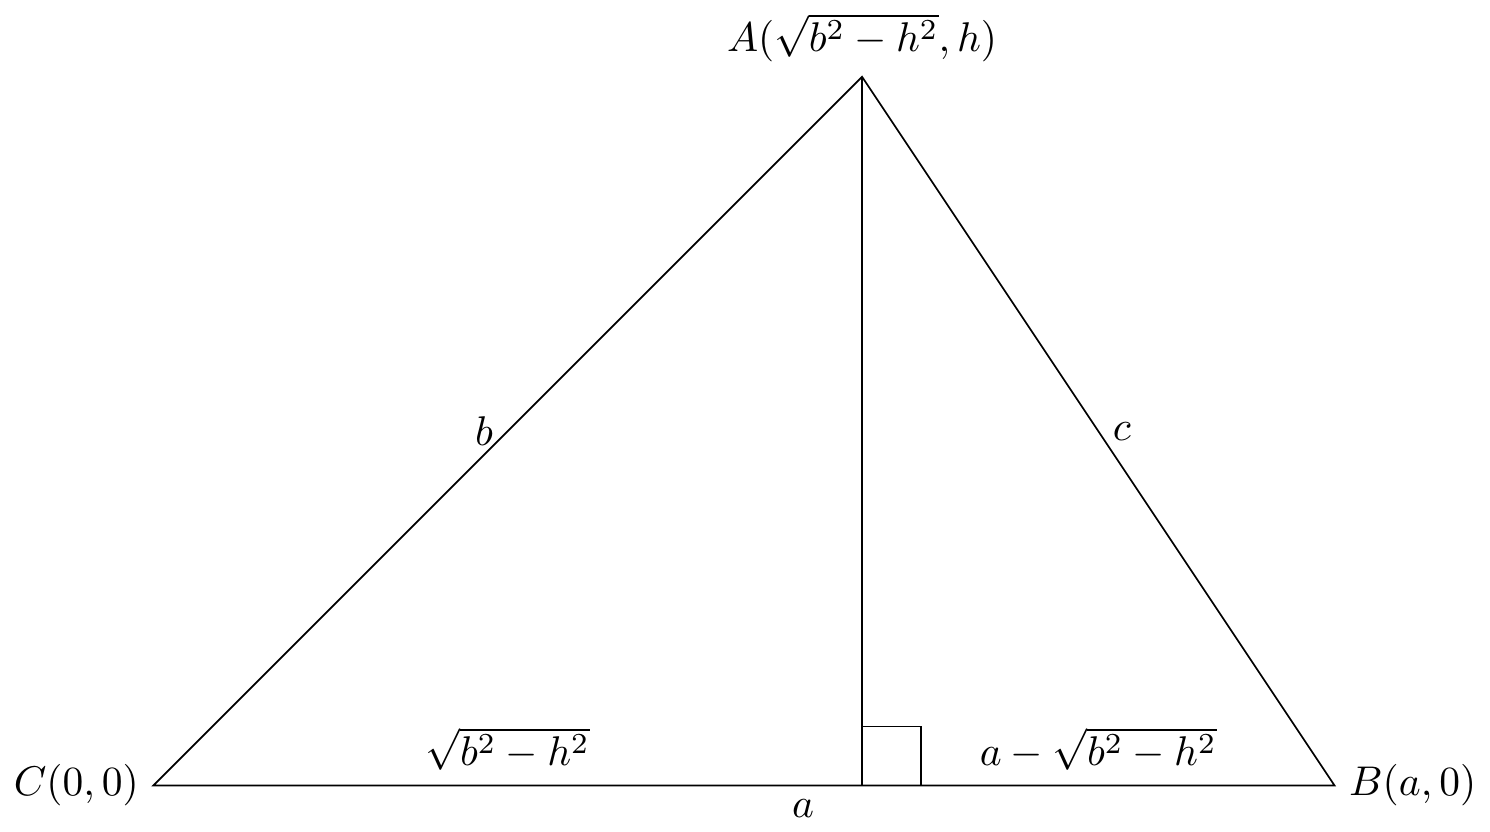
\includegraphics[width=1\linewidth,height=\textheight,keepaspectratio]{./figure/triangle.png}
\caption{Labelled triangle with one vertex at the origin.}
\end{figure}

--\textgreater{}\\
Here is a simple proof of Heron's formula using Cartesian geometry.

\[
\begin{aligned}
a - \sqrt{b^2 - h^2} &= \sqrt{c^2 - h^2} \\
(a - \sqrt{b^2 - h^2})^2 &= (\sqrt{c^2 - h^2})^2 \\
a^2 - 2a\sqrt{b^2 - h^2} + (b^2 - h^2) &= (c^2 - h^2) \\
a^2 + b^2 - h^2 - 2a\sqrt{b^2 - h^2} &= c^2 - h^2 \\
(a^2 + b^2 - c^2)^2 &= (2a\sqrt{b^2 - h^2})^2 \\
(a^2 + b^2 - c^2)(a^2 + b^2 - c^2) &= 4a^2(b^2 - h^2) \\
a^4 + b^4 + c^4 + 2a^2b^2 - 2a^2c^2 - 2b^2c^2 &= 4a^2b^2 - 4a^2h^2 \\
4a^2h^2 &= -a^4 - b^4 - c^4 - 2a^2b^2 + 4a^2b^2 + 2a^2c^2 + 2b^2c^2 \\
4a^2h^2 &= -a^4 - b^4 - c^4 + 2a^2b^2 + 2a^2c^2 + 2b^2c^2 \\
h &= \sqrt{\dfrac{-a^4 - b^4 - c^4 + 2a^2b^2 + 2a^2c^2 + 2b^2c^2}{4a^2}} \\
h &= \dfrac{1}{2a} \sqrt{-a^4 - b^4 - c^4 + 2a^2b^2 + 2a^2c^2 + 2b^2c^2} \\
\Delta &= \dfrac{1}{2} \times \text{base $\times$ height, where base $= a$} \\
\Delta &= \dfrac{1}{2} \times a \times \dfrac{1}{2a} \sqrt{-a^4 - b^4 - c^4 + 2a^2b^2 + 2a^2c^2 + 2b^2c^2} \\
\Delta &= \dfrac{1}{4} \sqrt{-a^4 - b^4 - c^4 + 2a^2b^2 + 2a^2c^2 + 2b^2c^2} \\
\Delta &= \dfrac{1}{4} \sqrt{-a^4 - b^4 - c^4 + 2a^2b^2 + 2a^2c^2 - 2b^2c^2 + 4b^2c^2} \\
\Delta &= \dfrac{1}{4} \sqrt{4b^2c^2 - (a^4 + b^4 + c^4 - 2a^2b^2 - 2a^2c^2 + 2b^2c^2)} \\
\text{Let}\; \alpha &= a^4 + b^4 + c^4 - 2a^2b^2 - 2a^2c^2 + 2b^2c^2 \\
&= a^4 + b^4 + c^4 - a^2b^2 - a^2b^2 - a^2c^2 - a^2c^2 + b^2c^2 \\
    &\qquad\quad + b^2c^2 \\
&= a^4 - a^2b^2 - a^2c^2 + b^4 - a^2b^2 + b^2c^2 + c^4 - a^2c^2 \\
    &\qquad\quad + b^2c^2 \\
&= a^2(a^2 - b^2 - c^2) + b^2(b^2 - a^2 + c^2) + c^2(c^2 - a^2 + b^2) \\
&= a^2(a^2 - b^2 - c^2) + b^2(-a^2 + b^2 + c^2) \\
        &\qquad\quad + c^2(-a^2 + b^2 + c^2) \\
&= -a^2(-a^2 + b^2 + c^2) + b^2(-a^2 + b^2 + c^2) \\
        &\qquad\quad + c^2(-a^2 + b^2 + c^2) \\
&= (-a^2 + b^2 + c^2)(-a^2 + b^2 + c^2) \\
\alpha &= (-a^2 + b^2 + c^2)^2
\end{aligned}
\]

\[
\begin{aligned}
\text{Thus,}\; \Delta &= \dfrac{1}{4} \sqrt{4b^2c^2 - (-a^2 + b^2 + c^2)^2} \\
\Delta &= \dfrac{1}{4} \sqrt{(2bc)^2 - (-a^2 + b^2 + c^2)^2} \\
\Delta &= \dfrac{1}{4} \sqrt{(2bc - (-a^2 + b^2 + c^2))(2bc + (-a^2 + b^2 + c^2))} \\
\Delta &= \dfrac{1}{4} \sqrt{(2bc + a^2 - b^2 - c^2)(2bc - a^2 + b^2 + c^2)} \\
\text{Let}\; m &= 2bc + a^2 - b^2 - c^2 \\
m &= a^2 - b^2 - c^2 + ab - ab + ac - ac + bc + bc \\
&= (a^2 + ac - ab) + (-b^2 + bc + ab) + (-c^2 + bc - ac) \\
&= a(a + c - b) - b(b - c - a) - c(c - b + a) \\
&= a(a + c - b) + b(a + c - b) - c(a + c - b) \\
m &= (a + b - c)(a + c - b) \\
\text{Let}\; n &= 2bc - a^2 + b^2 + c^2 \\
n &= -a^2 + b^2 + c^2 + ab - ab + ac - ac + bc + bc \\
&= (-a^2 + ac + ab) + (b^2 + bc - ab) + (c^2 + bc - ac) \\
&= a(-a + c + b) + b(b + c - a) + c(c + b - a) \\
&= a(b + c - a) + b(b + c - a) + c(b + c - a) \\
n &= (a + b + c)(b + c - a) \\
\Delta &= \dfrac{1}{4} \sqrt{mn} \\
&= \sqrt{\dfrac{mn}{16}} \\
&= \sqrt{\dfrac{(a + b - c)(a + c - b)(a + b + c)(b + c - a)}{16}} \\
&= \sqrt{\dfrac{a + b + c}{2} \times \dfrac{b + c - a}{2} \times \dfrac{a + c - b}{2} \times \dfrac{a + b - c}{2}} \\
&= \sqrt{\dfrac{a + b + c}{2} \times \dfrac{a + b + c - 2a}{2} \times \dfrac{a + b + c - 2b}{2} \times \dfrac{a + b + c - 2c}{2}} \\
&= \sqrt{\left(\dfrac{a + b + c}{2}\right) \times \left(\dfrac{a + b + c}{2} - a\right) \times \left(\dfrac{a + b + c}{2} - b\right) \times \left(\dfrac{a + b + c}{2} - c\right)} \\
\text{Let}\; S &= \dfrac{a + b + c}{2}, \\
\text{then}\; \Delta &= \sqrt{S(S - a)(S - b)(S - c)}
\end{aligned}
\]

\hfill\break
Heron's formula proved!

\bibliography{book.bib,packages.bib}

\end{document}
